\documentclass[conference]{IEEEtran}
\IEEEoverridecommandlockouts
% The preceding line is only needed to identify funding in the first footnote. If that is unneeded, please comment it out.
\usepackage{cite}
\usepackage{amsmath,amssymb,amsfonts}
\usepackage{algorithmic}
\usepackage{graphicx}
\usepackage{textcomp}
\usepackage{xcolor}
\usepackage[hyphens]{url} 
\usepackage{graphicx}
\usepackage{subfigure}
\usepackage{bibentry}
\usepackage{ragged2e}
%\usepackage{balance}
\usepackage{flushend}
\usepackage{booktabs,makecell,multirow,tabularx}
\urlstyle{rm} 
\def\UrlFont{\rm}  
\def\BibTeX{{\rm B\kern-.05em{\sc i\kern-.025em b}\kern-.08em
    T\kern-.1667em\lower.7ex\hbox{E}\kern-.125emX}}

\makeatletter % changes the catcode of @ to 11
\newcommand{\linebreakand}{%
  \end{@IEEEauthorhalign}
  \hfill\mbox{}\par
  \mbox{}\hfill\begin{@IEEEauthorhalign}
}
\makeatother % changes the catcode of @ back to 12

\begin{document}
%\title{Evaluation of Performance of Llama 2 Against Other LLMs}
%\title{Performance of Llama 2 Against Other LLMs}
\title{Performance Analysis of Llama 2 \\Among  Other LLMs}

%\author{
%\IEEEauthorblockN{1\textsuperscript{st} Donghao HUANG}
%\IEEEauthorblockA{\textit{School of Computing and Information Systems} \\
%\textit{Singapore Management University}\\
%Singapore, Singapore  \\
%dh.huang.2023@smu.edu.sg}
%\and

%\IEEEauthorblockN{2\textsuperscript{nd} Zhenda Hu}
%\IEEEauthorblockA{\textit{School of Information Management and Engineering} \\
%\textit{Shanghai University of Finance and Economics}\\
%Shanghai, China  \\
%huzhenda2020@gmail.com}
%\and

%\linebreakand
%\IEEEauthorblockN{3\textsuperscript{rd} Zhaoxia WANG}
%\IEEEauthorblockA{\textit{School of Computing and Information Systems} \\
%\textit{Singapore Management University}\\
%Singapore, Singapore  \\
%zxwang@smu.edu.sg}
%}
%\author{\IEEEauthorblockN{Anonymous Authors}}
\author{\IEEEauthorblockN{Donghao HUANG\textsuperscript{1,2},
Zhenda HU\textsuperscript{3},
Zhaoxia WANG\textsuperscript{1*}
%\IEEEauthorrefmark{1},
}


\IEEEauthorblockA{School of Computing and Information Systems, Singapore Management University, Singapore\textsuperscript{1}}
\IEEEauthorblockA{Research and Development, Mastercard, Singapore\textsuperscript{2}}
\IEEEauthorblockA{School of Information Management and Engineering, Shanghai University of Finance and Economics, Shanghai, China\textsuperscript{3}}
\IEEEauthorblockA{dh.huang.2023@smu.edu.sg; huzhenda2020@gmail.com; zxwang@smu.edu.sg*}
\thanks{\IEEEauthorrefmark{1}Corresponding Author: Zhaoxia WANG (e-mail: zxwang@smu.edu.sg)}
}
\maketitle

\begin{abstract}
Llama 2, an open-source large language model developed by Meta, offers a versatile and high-performance solution for natural language processing, boasting a broad scale, competitive dialogue capabilities, and open accessibility for research and development, thus driving innovation in AI applications. Despite these advancements, there remains a limited understanding of the underlying principles and performance of Llama 2 compared with other LLMs. To address this gap, this paper presents a comprehensive evaluation of Llama 2, focusing on its application in in-context learning — an AI design pattern that harnesses pre-trained LLMs for processing confidential and sensitive data. Through a rigorous comparative analysis with other open-source LLMs and OpenAI models, this study sheds light on Llama 2's performance, quality, and potential use cases. Our findings indicate that Llama 2 holds significant promise for applications involving in-context learning, with notable strengths in both answer quality and inference speed.
This research offers valuable insights for the fields of LLMs and serves as an effective reference for companies and individuals utilizing such large models.
%However, considerations for licensing terms and scalability are paramount for large enterprises seeking to harness the power of this open-source technology.
The source codes and datasets of this paper are accessible at \url{https://github.com/inflaton/Llama-2-eval}.
\end{abstract}

\begin{IEEEkeywords}
large language model, in-context learning, generative pre-trained transformer, model evaluation
\end{IEEEkeywords}

\section{Background and Introduction}
On July 18, 2023, Meta announced the release of Llama 2, the next generation of their open-source large language model (LLM) \cite{touvron2023llama}. Llama 2 is available for both research and commercial use, with Microsoft as its preferred partner. This open-source model serves as a foundational AI technology that empowers businesses and developers to create advanced applications such as chatbots and personal assistants, which require the generation of human-like text. It offers a solution for organizations that may lack the resources to develop such complex models from scratch.

According to the official Hugging Face organization for Llama 2 models from Meta \footnote{\url{https://huggingface.co/meta-llama}}, Llama 2 comprises pretrained and fine-tuned generative text models ranging from 7 billion to 70 billion parameters among these models, Llama-2-Chat has been specifically optimized for dialogue-based use cases \cite{touvron2023llama}. Notably, Llama-2-Chat models excel in open-source chat model benchmarks and receive favorable evaluations in terms of helpfulness and safety, rivaling some well-known closed-source models like ChatGPT \cite{wang2023cost, adlakha2023evaluating} and PaLM \cite{wang2023pandalm}.


Upon Meta's announcement, we promptly submitted a request for a commercial license, which was granted shortly. This license enables us to conduct comprehensive comparisons between Llama 2 models and other large language models (LLMs).
%The release of Llama 2 represents a significant milestone in the fields of artificial intelligence and natural language processing (NLP). 
%Developed by Meta, Llama 2 offers a versatile platform for innovative AI applications. 
This paper delves into the capabilities of Llama 2, with a particular emphasis on its role in in-context learning — an emerging AI design pattern that harnesses pretrained LLMs to process confidential and sensitive data. We have made the following contributions:

\begin{itemize}
    \item Developed unique metrics and methodologies to assess the in-context learning of Llama 2 against various LLMs. 
    \item Performed an in-depth comparison of Llama-2 models with other top-tier LLMs, emphasizing their in-context learning strengths.
    \item Beyond corroborating Meta’s claims about Llama-2's capabilities, we've highlighted its commercial potential and offered insights for seamless enterprise adoption. 
\end{itemize}


\section{Related Work}

In recent years, the rapid advancement of large language models (LLMs) has transformed the landscape of natural language processing (NLP) and artificial intelligence (AI). With the introduction of Llama 2 \cite{touvron2023llama}, there has been a surge of interest in evaluating and harnessing its capabilities. In this section, we review related work that contextualizes our comprehensive evaluation of Llama 2 and its implications for AI applications, with a particular focus on in-context learning.

\subsection{Advances in Large Language Models}
The development of LLMs has been a focal point of research and innovation in the field of NLP \cite{kamalloo2023evaluating, sharir2020cost, xu2022survey}. LLMs have a great deal of potential as capable AI assistants that can carry out complex reasoning tasks in a variety of disciplines. Due to the ease with which they may promote human engagement through user-friendly chat interfaces, they have been quickly and widely accepted by the general public. 
Notable models like GPT-3 and others have demonstrated the potential of pre-trained LLMs in various applications, ranging from text generation to translation and dialogue systems \cite{wang2023cost, xu2022survey}. 

Our work builds upon this body of research by assessing the unique qualities of Llama 2, specifically in the context of in-context learning, and comparing it with existing LLMs.

\subsection{In-Context Learning and Pre-trained LLMs}
In-context learning, as an AI design pattern, has gained prominence for its ability to process confidential and sensitive data using pre-trained LLMs \cite{min2022rethinking}. Prior studies have explored the use of LLMs for handling contextually relevant information and generating context-aware responses \cite{cai2022context}. 
We aim to contribute to this area of research by providing a comprehensive evaluation of Llama 2's performance and suitability for in-context learning, shedding light on its strengths and potential use cases.

\subsection{Comparative Analyses of LLMs}
Comparative analyses of LLMs have been instrumental in assessing their capabilities and identifying their relative advantages. Existing research has compared different LLMs on various benchmarks, considering factors such as answer quality \cite{chen2023exploring}\cite{huang2024evaluation}, inference speed \cite{huang2024evaluation}\cite{zheng2023response}, and safety \cite{zhang2023safetybench}. 
Our study aligns with this research theme, as we conduct a rigorous comparative analysis between Llama 2 and other open-source LLMs and OpenAI models, aiming to provide insights into its competitive edge and unique contributions.

%The subsequent sections of this paper delve into technique approach and methodology, results and discussions, and conclusions of our study, further illuminating the significance of Llama 2 in the field of NLP and AI and filling a crucial gap in our understanding of its capabilities.


\section{Methodology}
In this section, we present our approach and methodology for the comprehensive evaluation of Llama 2, with a specific focus on its application in in-context learning, as well as its comparison with existing large language models (LLMs). Our methodology encompasses data collection and preprocessing, model selection, in-context learning workflow and evaluation metrics.

%\subsection{In-Context Learning}
%Our methodology is deeply rooted in the "In-Context Learning" design paradigm. This model leverages existing Large Language Models (LLMs) without the necessity for additional fine-tuning. Instead, it manipulates model behaviors using targeted prompting and conditions them on private "contextual" data, like text from PDF files. This ensures that generative AI technologies process confidential information securely, either locally or within an enterprise's IT framework. Our in-context learning methodology unfolds in three clear stages, as illustrated in Figure \ref{fig:1}:

%\begin{enumerate}[(1)]
   % \item Data Processing and Embedding: Here, confidential documents are archived for future reference. Typically, these documents are broken down into smaller segments, run through an embedding model, and the resulting embeddings are stored in a vector repository.
   % \item Prompt Creation and Retrieval: On receiving a user query, the system formulates and sends a series of prompts to the language model. A finalized prompt combines a base template with relevant documents from the vector repository. Notably, when prior chat interactions exist, the LLM crafts standalone queries to enhance retrieval, highlighted in subsequent tables.
   % \item Prompt Execution and Inference: After prompt assembly, they're dispatched to a pre-trained LLM for decision-making. This encompasses both proprietary model interfaces and those that are open-sourced or self-trained. 
%\end{enumerate}

%\begin{figure*}
%\centering
%  \includegraphics[width=1.0\textwidth]{Figure1.png}
  %\includegraphics[width=1\textwidth]{Fig1.png}
% figure caption is below the figure
%\caption{In-Context Learning Workflow}
%\label{fig:1}       % Give a unique label
%\end{figure*}

By adopting this systematic approach, we harness in-context learning's potential, ensuring efficient and secure interactions with Large Language Models.

\subsection{Data Collection and Preprocessing}
To rigorously evaluate Llama 2's capabilities, we employed a subset of the MS MARCO dataset, a comprehensive reading comprehension and question answering dataset curated by Microsoft \footnote{\url{https://github.com/microsoft/MSMARCO-Question-Answering\#qa}}. We carefully handpicked 100 queries with well-formed answers across five categories (LOCATION, NUMERIC, PERSON, DESCRIPTION, ENTITY), resulting in a test dataset comprising 500 queries. Table \ref{dataset-overview} provides an overview of this evaluation dataset.

%\begin{figure*}
%\centering
%  \includegraphics[width=0.8\textwidth]{Figure2.png}
% figure caption is below the figure
%\caption{MS MACRO-based Evaluation Dataset (code snippets from: https://github.com/inflaton/Llama-2-eval/blob/master/notebook/metrics.ipynb)}
%\label{fig:2}       % Give a unique label
%\end{figure*}

\begin{table*}
    \renewcommand{\arraystretch}{1.5}
    \centering
    \caption{Overview of Evaluation Dataset}
    \label{tab:the_table}
    \begin{tabular}{|p{5mm}|p{25mm}|p{25mm}|p{25mm}|p{16mm}|p{20mm}|p{34mm}|}
        \hline
         ID & Answers & Passages & Query & Query ID & Query Type & Well Formed Answers \\
        \hline
        0 & \lbrack 2,662\rbrack & \{'is\_selected': \lbrack 0, 0, 0, 1, 0, 0, 0, 0\rbrack, 'pas... & albany mn population & 15177 & NUMERIC & \lbrack The population of Albany, Minnesota is 2,662. \rbrack \\
        \hline
        %1 & \lbrack Hippocrates \rbrack  & \{'is\_selected': \lbrack 0, 0, 0, 0, 0, 1, 0, 0, 0, 0 \rbrack ... & \_\_\_\_\_\_\_\_\_\_ is considered the father ... & 9083 & DESCRIPTION & \lbrack Hippocrates is considered the father of moder...\\
        %\hline
%2 & \lbrack 120 days from the date of the Note. \rbrack  & \{'is\_selected': \lbrack 0, 1, 0, 0, 0, 0, 0, 0, 0, 0 \rbrack ... & how many days is an appraisal good for a fanni... & 281439 & NUMERIC & \lbrack An appraisal is good for 120 days from the da...\\
%        \hline
... & ... & ... & ... & ... & ... & ...\\
%        \hline
%497 & \lbrack Mount Able Baptist Church is located at the a... & \{'is\_selected': \lbrack 1, 0, 0, 0, 0, 0, 0, 0, 0 \rbrack , '... & mt. view baptist in pendleton sc & 460250 & PERSON & \lbrack Mount Able Baptist Church is located at the a...\\
        \hline
%498 & \lbrack Honeysuckle Weeks \rbrack  & \{'is\_selected': \lbrack 0, 0, 0, 1, 0, 0, 0, 0, 0, 0 \rbrack ... & what actress disappeared for a while & 549739 & PERSON & \lbrack The actress disappeared for a while Honeysuck...\\
%        \hline
499 & \lbrack African-Nguni \rbrack  & \{'is\_selected': \lbrack 0, 0, 1, 0, 0, 0, 0, 0 \rbrack , 'pas... & what ethnicity is the surname sabol & 658265 & PERSON & \lbrack The ethnicity of the surname Sabol is African...\\
        \hline

    \end{tabular}
\label{dataset-overview}  
\end{table*}

\subsection{Model Selection}
We purposefully chose our models to ensure a thorough comparative study. Llama 2 was our primary focus given its recent emergence and the notable features discussed in the related work section. Alongside it, we evaluated established LLMs like GPT-4, GPT-3.5, and several leading open-source models. However, due to our GPU cluster's memory constraints (48GB), we restricted our evaluation to open-source LLMs with up to 13B parameters. This selection framework was designed to benchmark Llama 2 against recognized standards, helping us discern its distinctive value in the domain.

\subsection{Experiment Setup}
To assess the in-context learning proficiency of chosen LLMs, we crafted a Python application leveraging LangChain \footnote{\url{https://github.com/langchain-ai/langchain}}, a renowned open-source platform tailored for seamless integration with LLMs. For each query in our evaluation set, the program creates a prompt that combines the query with its associated 10 passages for context. This prompt is forwarded to the LLM to produce a response. The generated answer is then compared with the established ground truth to assess its accuracy. Table \ref{query-processing} provides a visual representation of this process using sample data from a specific query.

Upon processing all 500 queries, the application computes various evaluation metrics, details of which are elucidated in the ensuing section. 
%For those interested in a deeper dive, both the program's source code and the MS MACRO-inspired evaluation dataset are accessible on GitHub at \url{https://github.com/inflaton/Llama-2-eval}.

\begin{table*}
    \renewcommand{\arraystretch}{1.5}
    \centering
    \caption{Steps of Processing a Query}
    \label{tab:the_table}
    \begin{tabular}{|p{40mm}|p{120mm}|}
        \hline
        1) Retrieve Query & \_\_\_\_\_\_\_\_\_\_\_\_\_\_\_\_\_\_\_\_ is considered the father of modern medicine.  \\
        \hline
        2) Create Prompt\newline and Send it to LLM & System: Use the following pieces of context to answer the users question. 
If you don't know the answer, just say that you don't know, don't try to make up an answer.\newline
----------------\newline
(... 10 passages inserted here as context ...)\newline
Human: \_\_\_\_\_\_\_\_\_\_\_\_\_\_\_\_\_\_\_\_ is considered the father of modern medicine.  \\
        \hline
        3) Compare LLM Generated Answer against Ground Truth & \textbf{\textit{Answer}}: Hippocrates is considered the father of modern medicine.  \newline 
        \newline 
        \textbf{\textit{Ground truth}}: Hippocrates is considered the father of modern medicine.  \\
        \hline
        
    \end{tabular}
\label{query-processing}  
\end{table*}

\iffalse
\begin{table*}
    \centering
    \caption{Steps of Processing a Query}
    \label{tab:the_table}
    \begin{tabular}{|p{30mm}|p{130mm}|}
        \hline
        1) Retrieve Query & \_\_\_\_\_\_\_\_\_\_\_\_\_\_\_\_\_\_\_\_ is considered the father of modern medicine.  \\
        \hline
        2) Create Prompt\newline and Send it to LLM & System: Use the following pieces of context to answer the users question. 
If you don't know the answer, just say that you don't know, don't try to make up an answer.\newline
----------------\newline
Hippocrates is widely considered to be the Father of Medicine. His contributions revolutionized the practice of medicine; but after his death the advancement stalled.\newline
\newline
Many of the invaluable lessons prescribed in that place of learning are assigned to Hippocrates. If that was the case, then it truly was Hippocrates, with his approach to healing and the role of the doctor, that influenced western medicine for thousands of years.\newline
\newline
Despite this, Hippocrates is attributed with a great many wonderful deeds and thoughts. He is recognised as the founder of the Hippocratic School of Medicine, a college that revolutionized the understanding of medicine in Ancient Greece.\newline
\newline
At least that is what we’d like to think. While his fame was such to warrant a mention from the likes of Plato and Aristotle, not much is actually known about Hippocrates the father of Medicine. Consequently, he has become the projection of what people ideally want in a physician.\newline
\newline
460 – c. 370 BC) was a Greek physician of the Age of Pericles (Classical Greece), and is considered one of the most outstanding figures in the history of medicine.\newline
\newline
TRUE. Hippocrates is considered the father of modern medicine because he did not believe that illness was a punishment inflicted by the gods. True False. Weegy: TRUE. [ \newline
\newline
The two sons of Hippocrates, Thessalus and Draco, and his son-in-law, Polybus, were his students. According to Galen, a later physician, Polybus was Hippocrates' true successor, while Thessalus and Draco each had a son named Hippocrates.\newline
\newline
Hippocrates is mentioned in passing in the writings of two contemporaries: Plato, in Protagoras and Phaedrus, and, Aristotle 's Politics, which date from the 4th century BC. Soranus wrote that Hippocrates' father was Heraclides, a physician, and his mother was Praxitela, daughter of Tizane.\newline
\newline
Reload the page to try again! Press Cmd-0 to reset your zoom. Press Ctrl-0 to reset your zoom. It looks like your browser might be zoomed in or out. Your browser needs to be zoomed to a normal size to record audio.\newline
\newline
However, the achievements of the writers of the Corpus, the practitioners of Hippocratic medicine, and the actions of Hippocrates himself were often commingled; thus very little is known about what Hippocrates actually thought, wrote, and did.\newline
Human: \_\_\_\_\_\_\_\_\_\_\_\_\_\_\_\_\_\_\_\_ is considered the father of modern medicine.  \\
        \hline
        3) Compare LLM Generated Answer against Ground Truth & \textbf{\textit{Answer}}: Hippocrates is considered the father of modern medicine.  \newline 
        \newline 
        \textbf{\textit{Ground truth}}: Hippocrates is considered the father of modern medicine.  \\
        \hline
        
    \end{tabular}
\label{query-processing}  
\end{table*}
\fi

\subsection{Evaluation Metrics}
When appraising the performance of Llama 2 and its counterparts, we adopted a suite of metrics specifically designed for in-context learning evaluations: 
\begin{itemize}
    \item Inference Speed: This metric gauges the rapidity of the models in processing queries and generating outputs, a pivotal attribute for applications necessitating real-time responses. It's quantified in terms of tokens generated per second.
    \item Answer Quality: A measure of the precision and pertinence of the answers produced by the models in the realm of in-context learning. Aligning with the official benchmarks for Question Answering and Natural Language Generation tasks \footnote{\url{https://microsoft.github.io/msmarco/}}, we opted for Rouge-L~\cite{lin2004rouge,joshi2023deepsumm} and Bleu-1~\cite{dey2022evaluating} to assess answer quality.
    
\end{itemize}

\section{Results and Discussions}
In this section, we showcase the results of our in-depth comparison between Llama 2 and other prominent LLMs, especially those from OpenAI. Our analysis covers aspects such as answer quality and inference speed, and we explore their relevance in the context of in-context learning applications.

\subsection{Inference Speed}
We evaluated inference speeds by running our test program on Nvidia A40 and L40 GPUs for Llama-2 and various open-source models. To optimize costs, we restricted testing of OpenAI models to the A40. Figure \ref{fig:5} presents the results, highlighting that the newer L40 GPU enhances inference speed by 24\% to 49\%, contingent on the LLM in use.

\begin{figure*}
\centering
  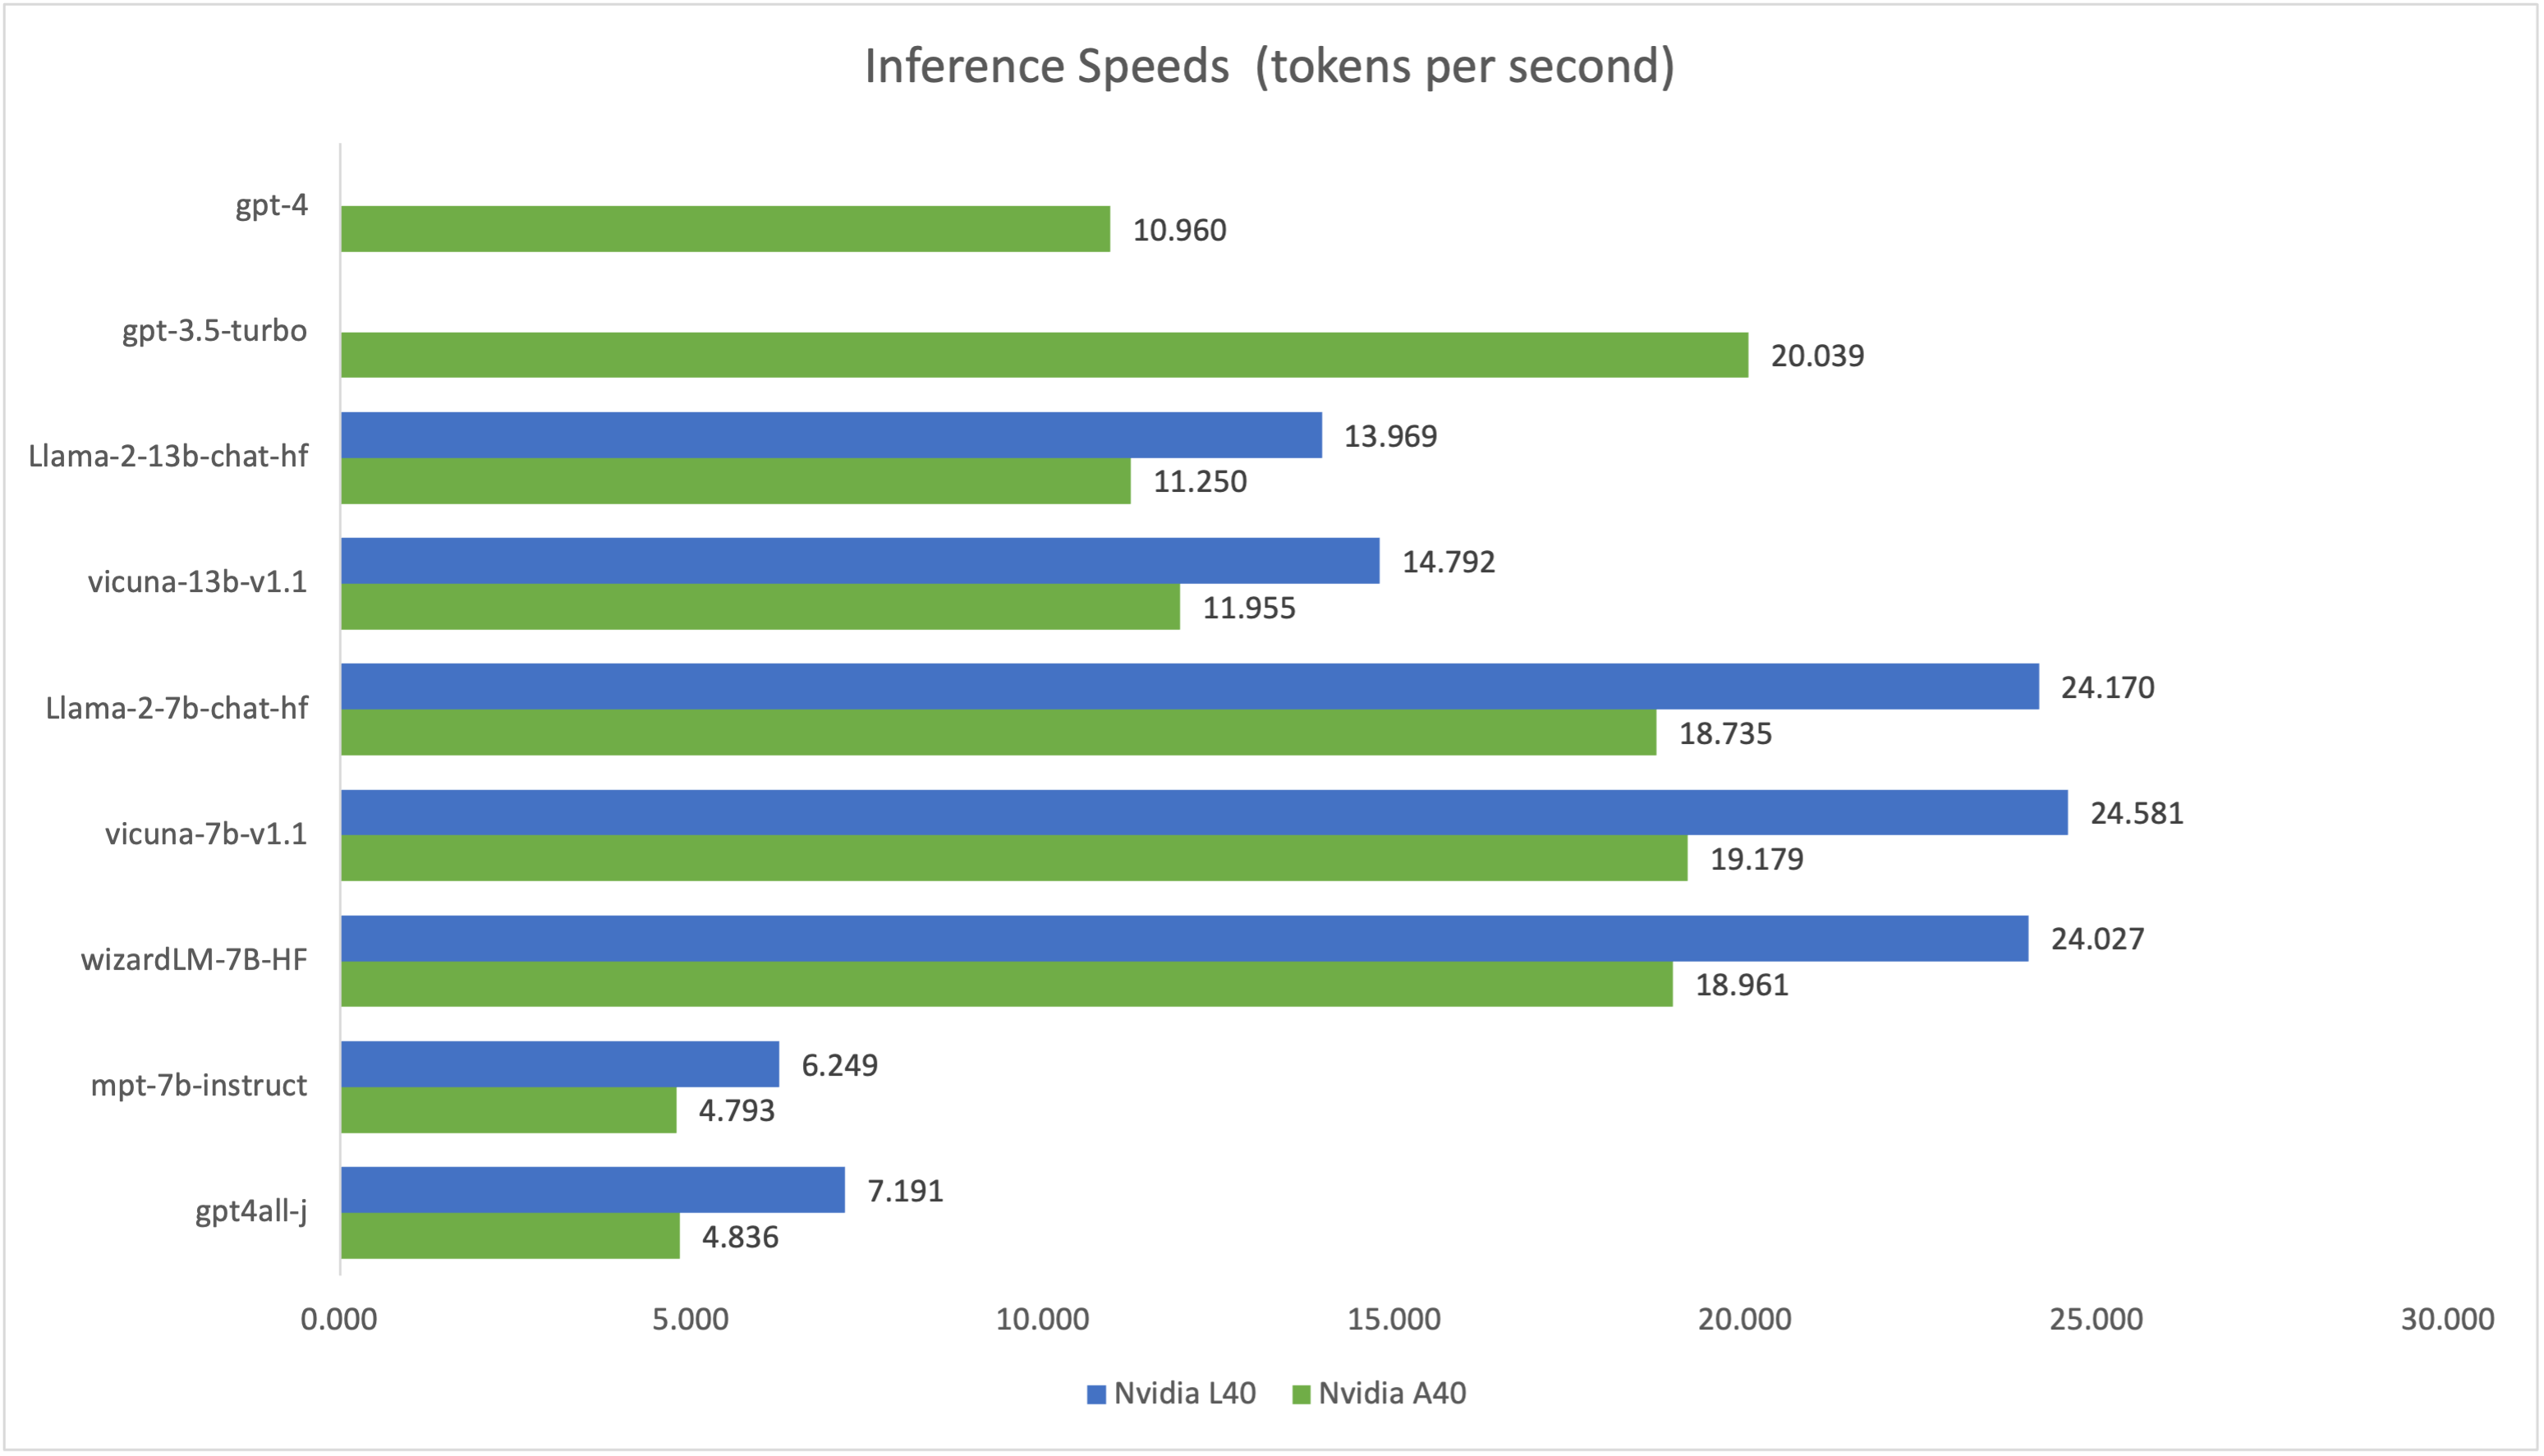
\includegraphics[width=0.80\textwidth]{figures/speed.png}
% figure caption is below the figure
\caption{Inference Speeds (running on Nvidia A40 and L40 GPUs)}
\label{fig:5}       % Give a unique label
\end{figure*}


\subsection{Answer Quality}
Figure \ref{fig:6} displays the answer quality metrics, specifically Rouge-L~\cite{lin2004rouge,joshi2023deepsumm} and Bleu-1~\cite{dey2022evaluating} scores, both overall and for each of the five categories: LOCATION, NUMERIC, PERSON, DESCRIPTION, and ENTITY. A notable observation is that while there are performance variations between different LLMs, all models consistently exhibit superior performance for queries in the LOCATION category compared to the others.

\begin{figure*}
\centering
    \subfigure[OVERALL]{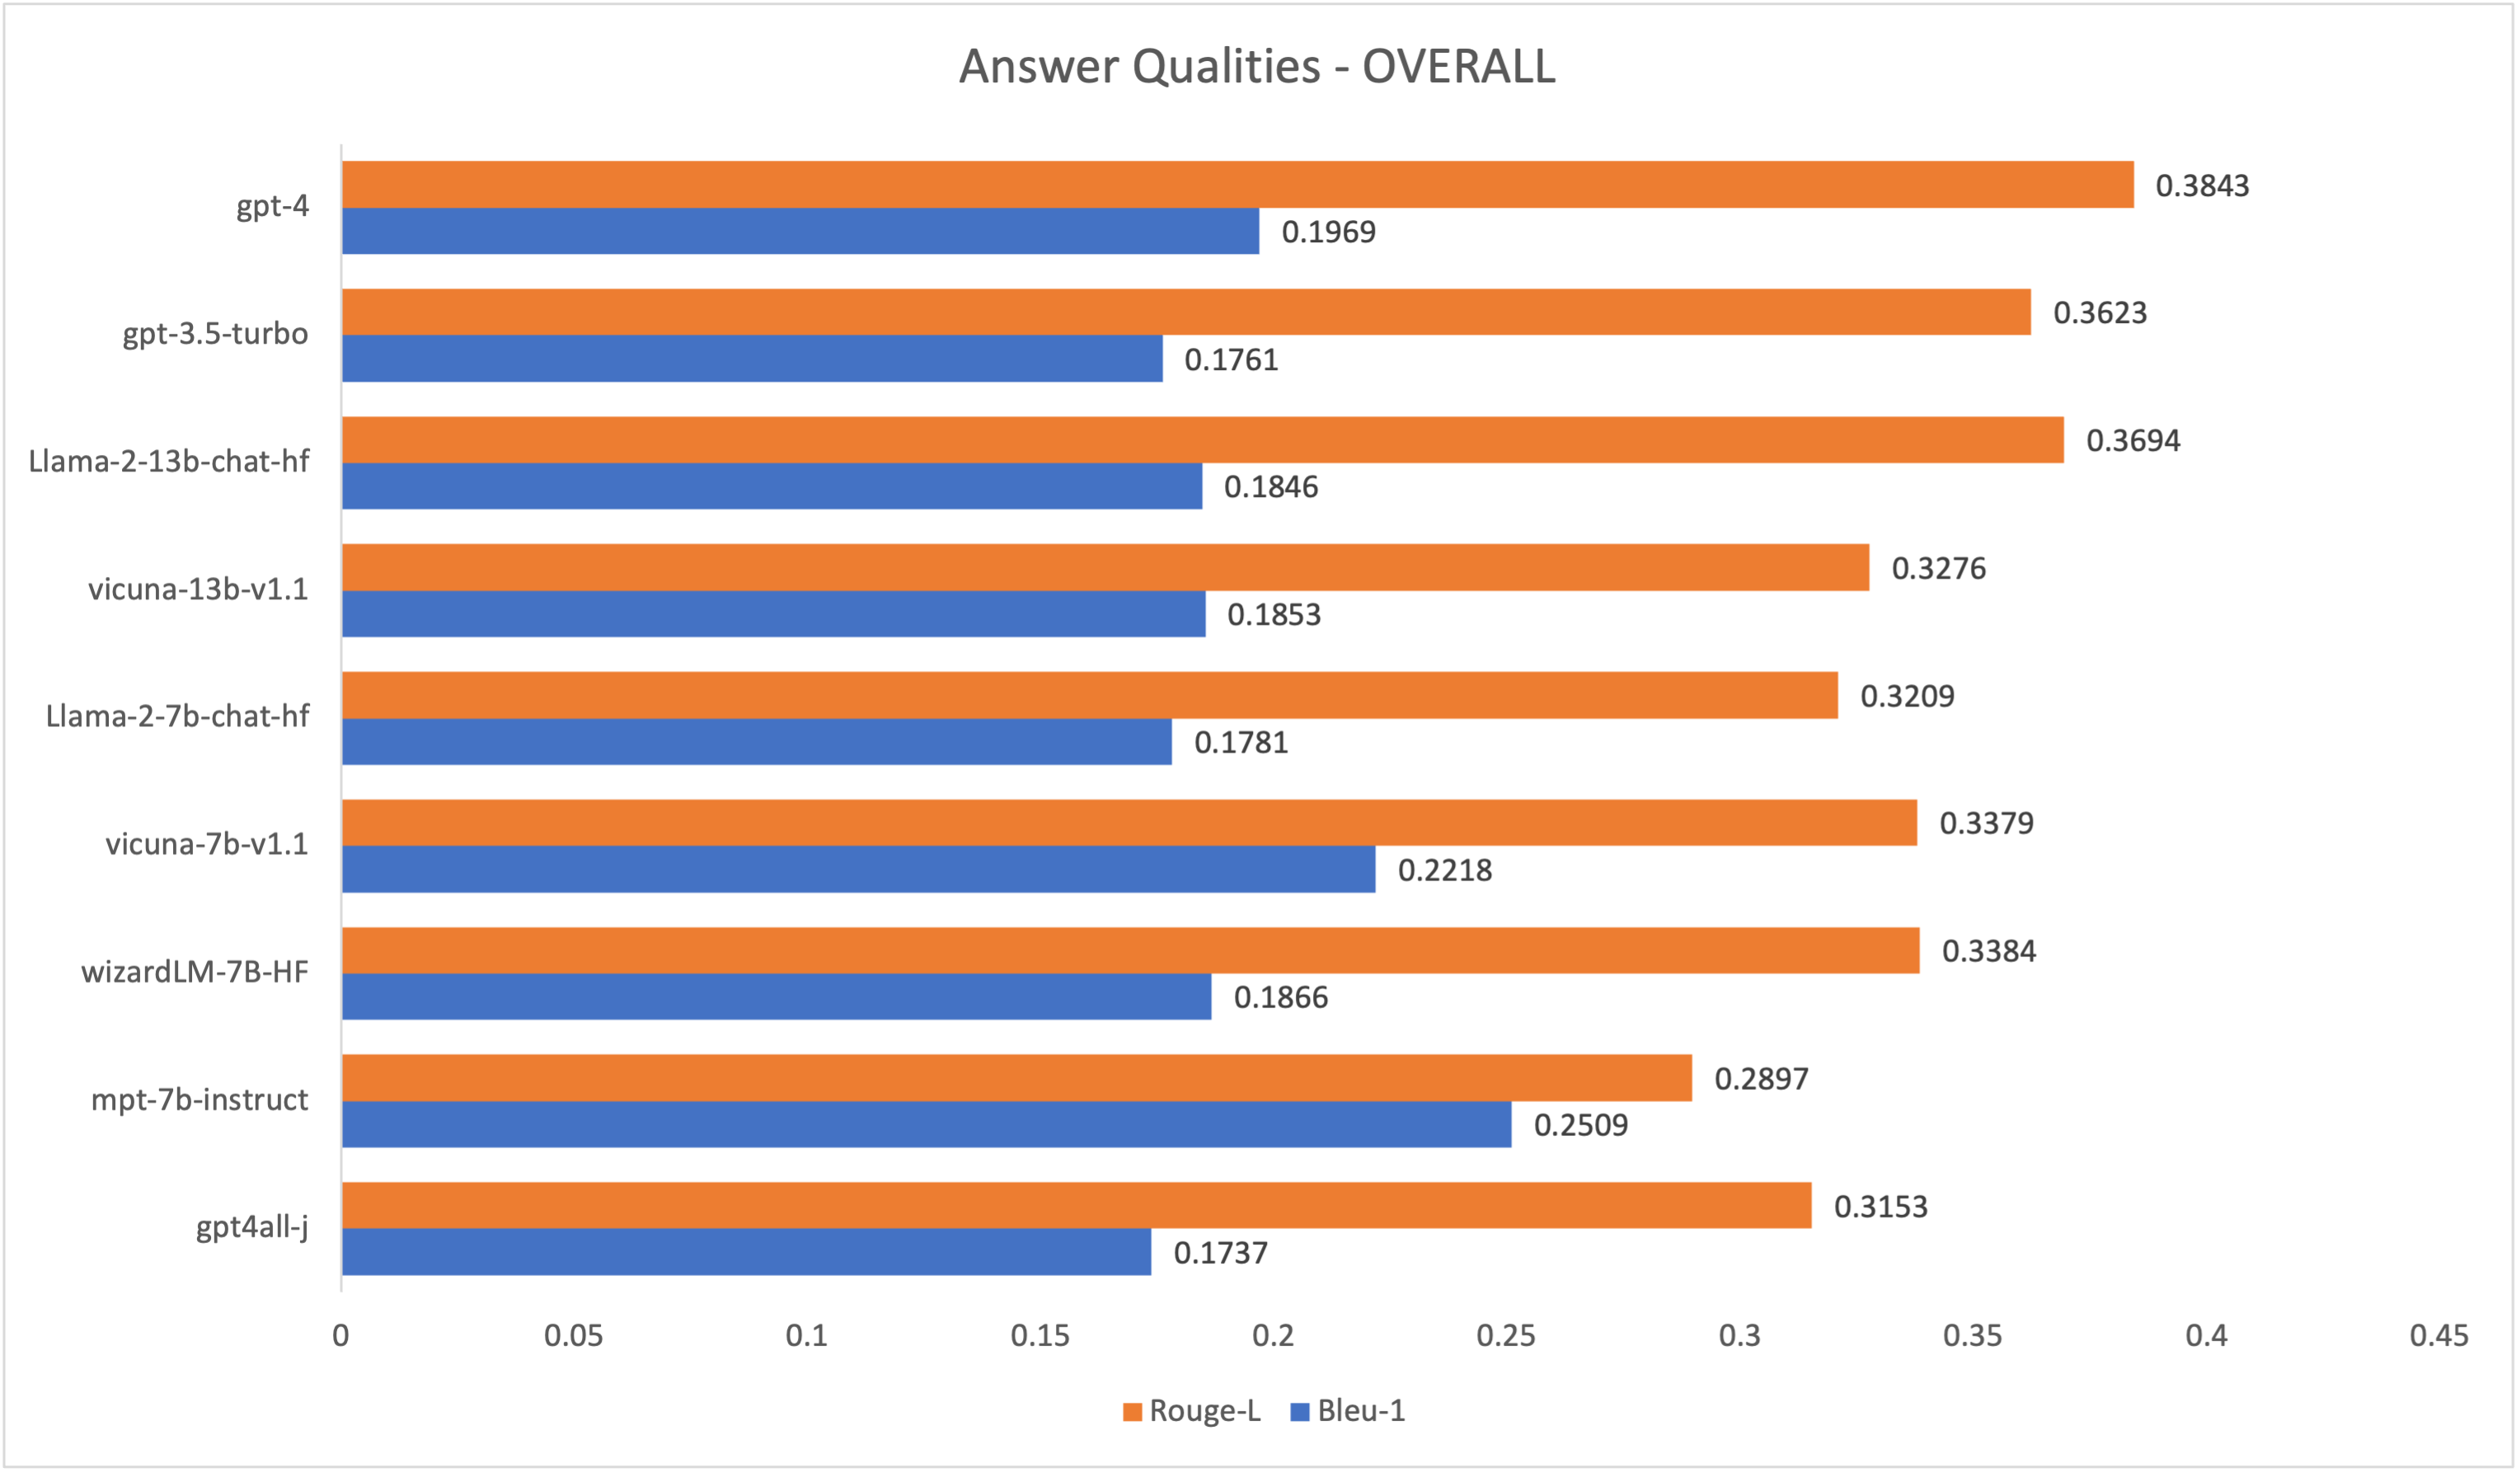
\includegraphics[width=0.48\textwidth]{figures/quality-overall.png}} 
    \subfigure[LOCATION]{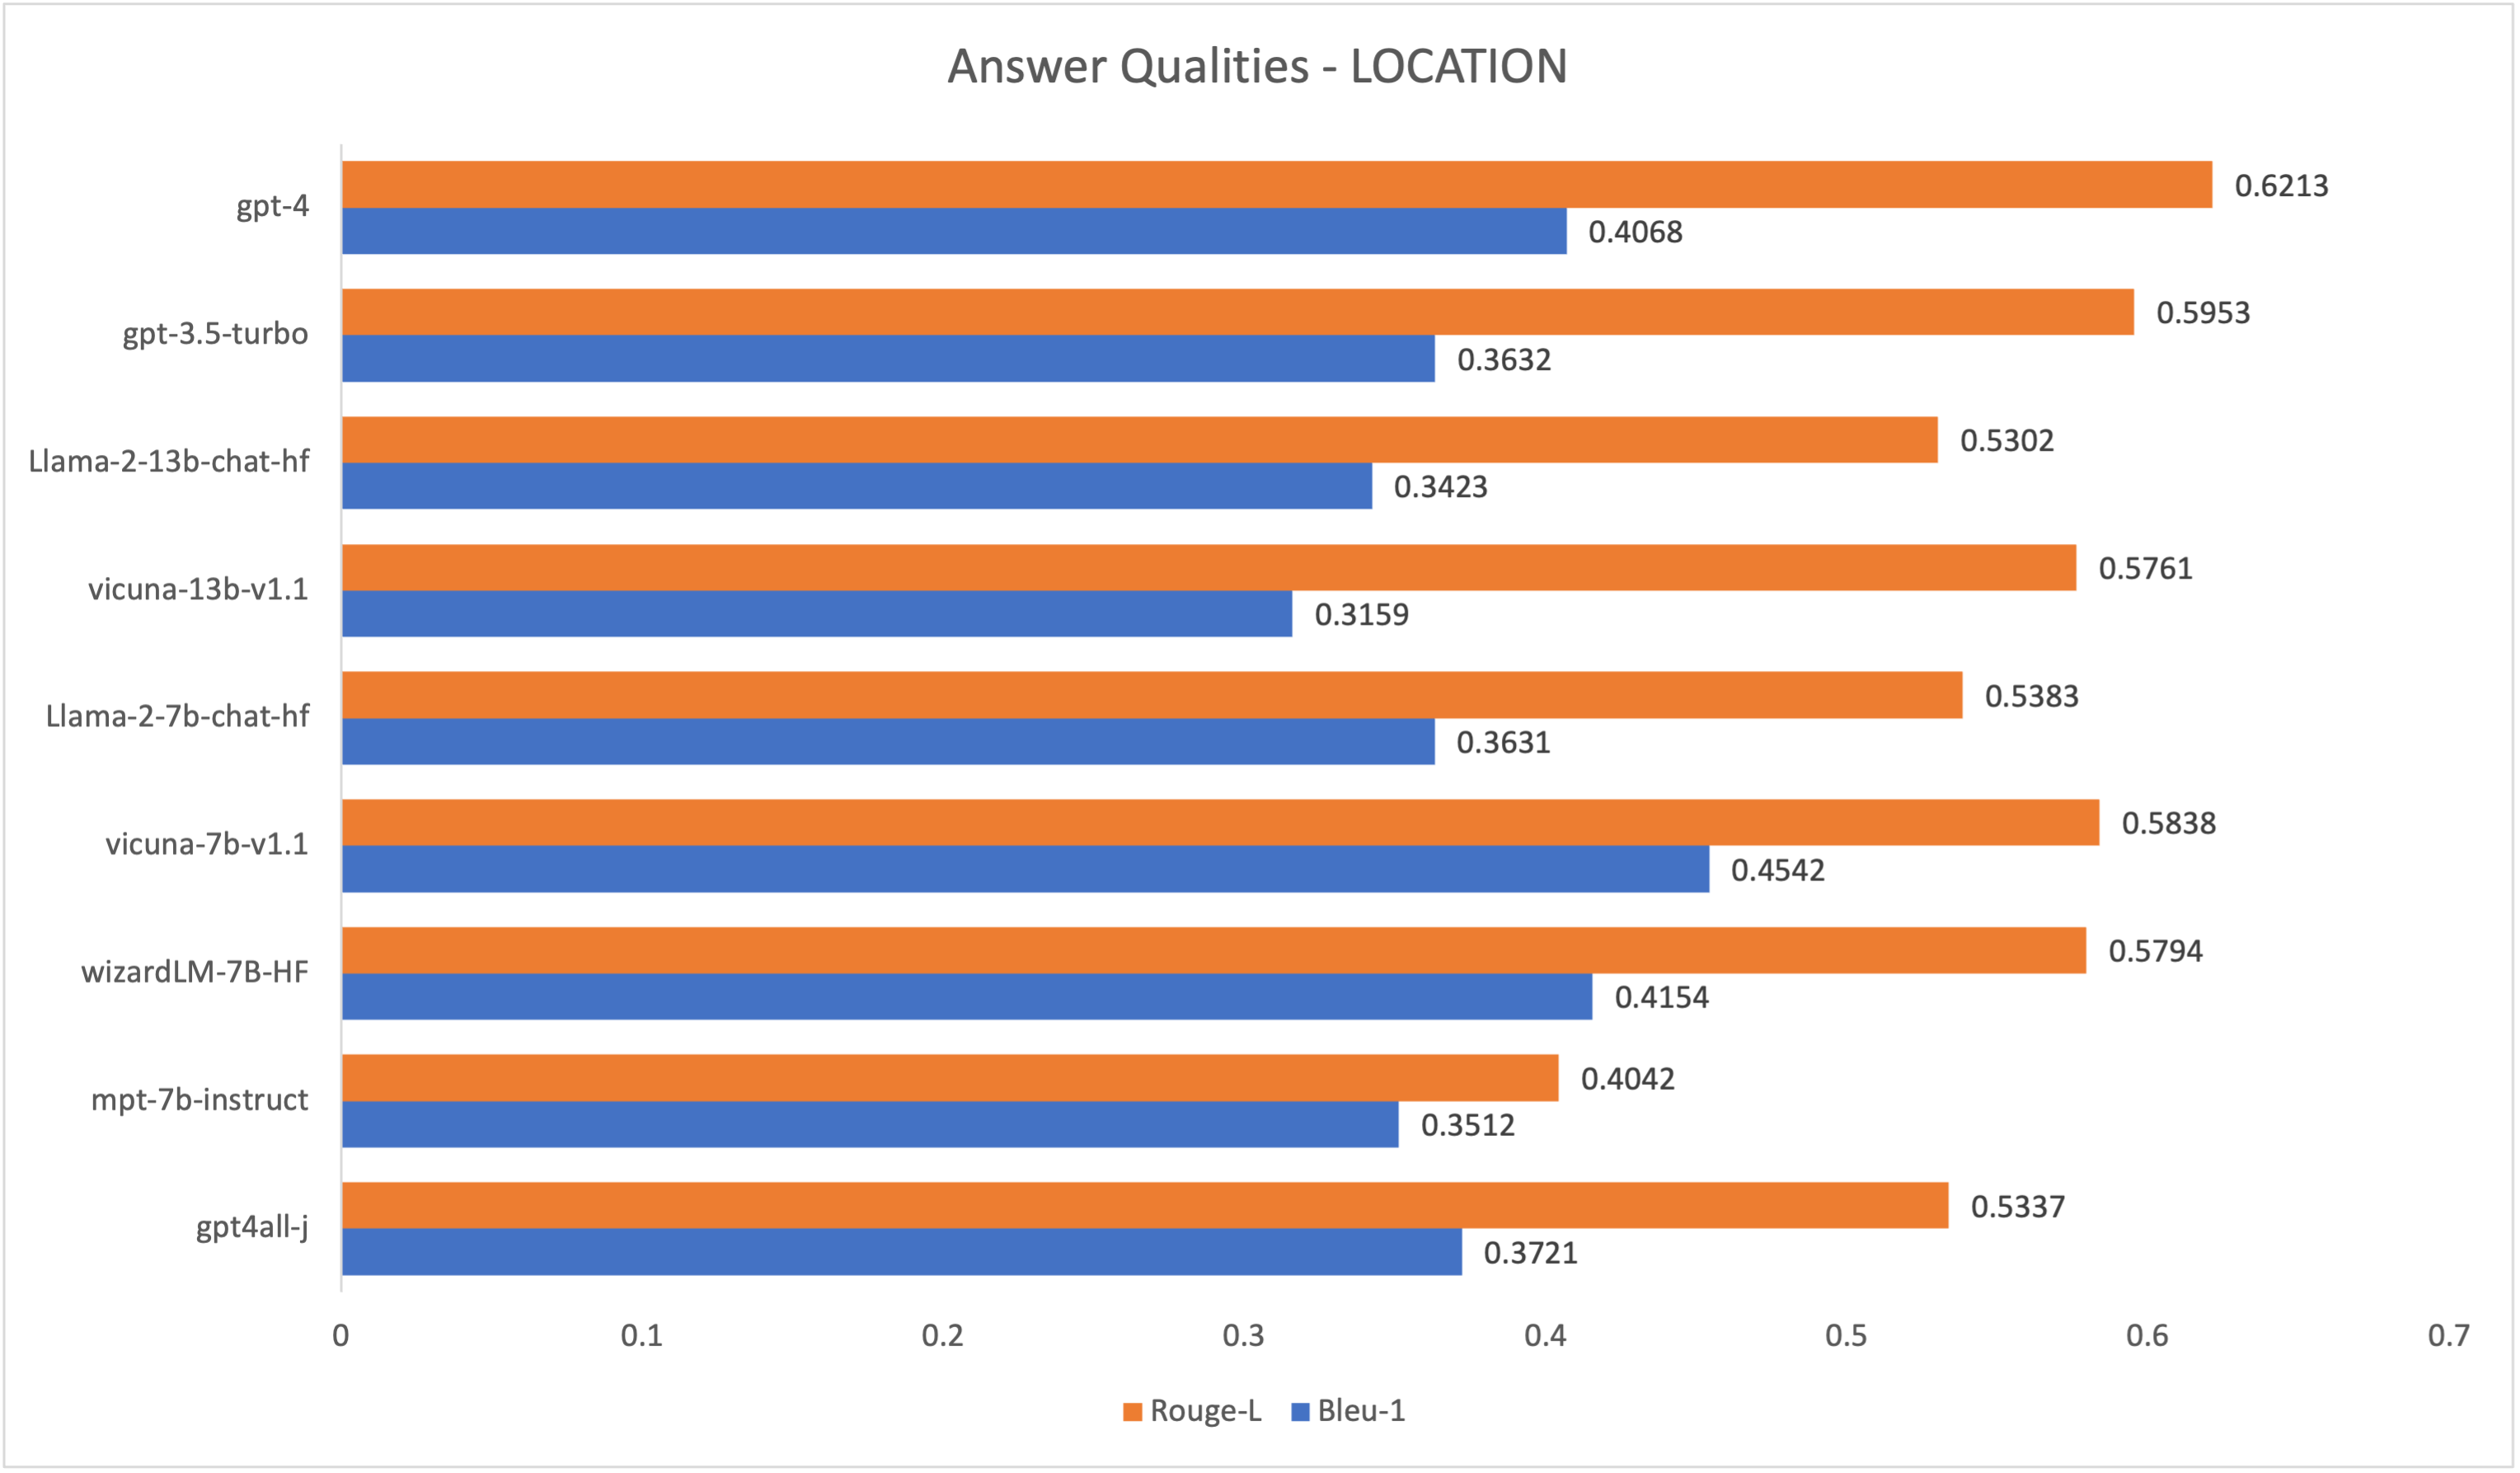
\includegraphics[width=0.48\textwidth]{figures/quality-location.png}} \\
    \subfigure[NUMERIC]{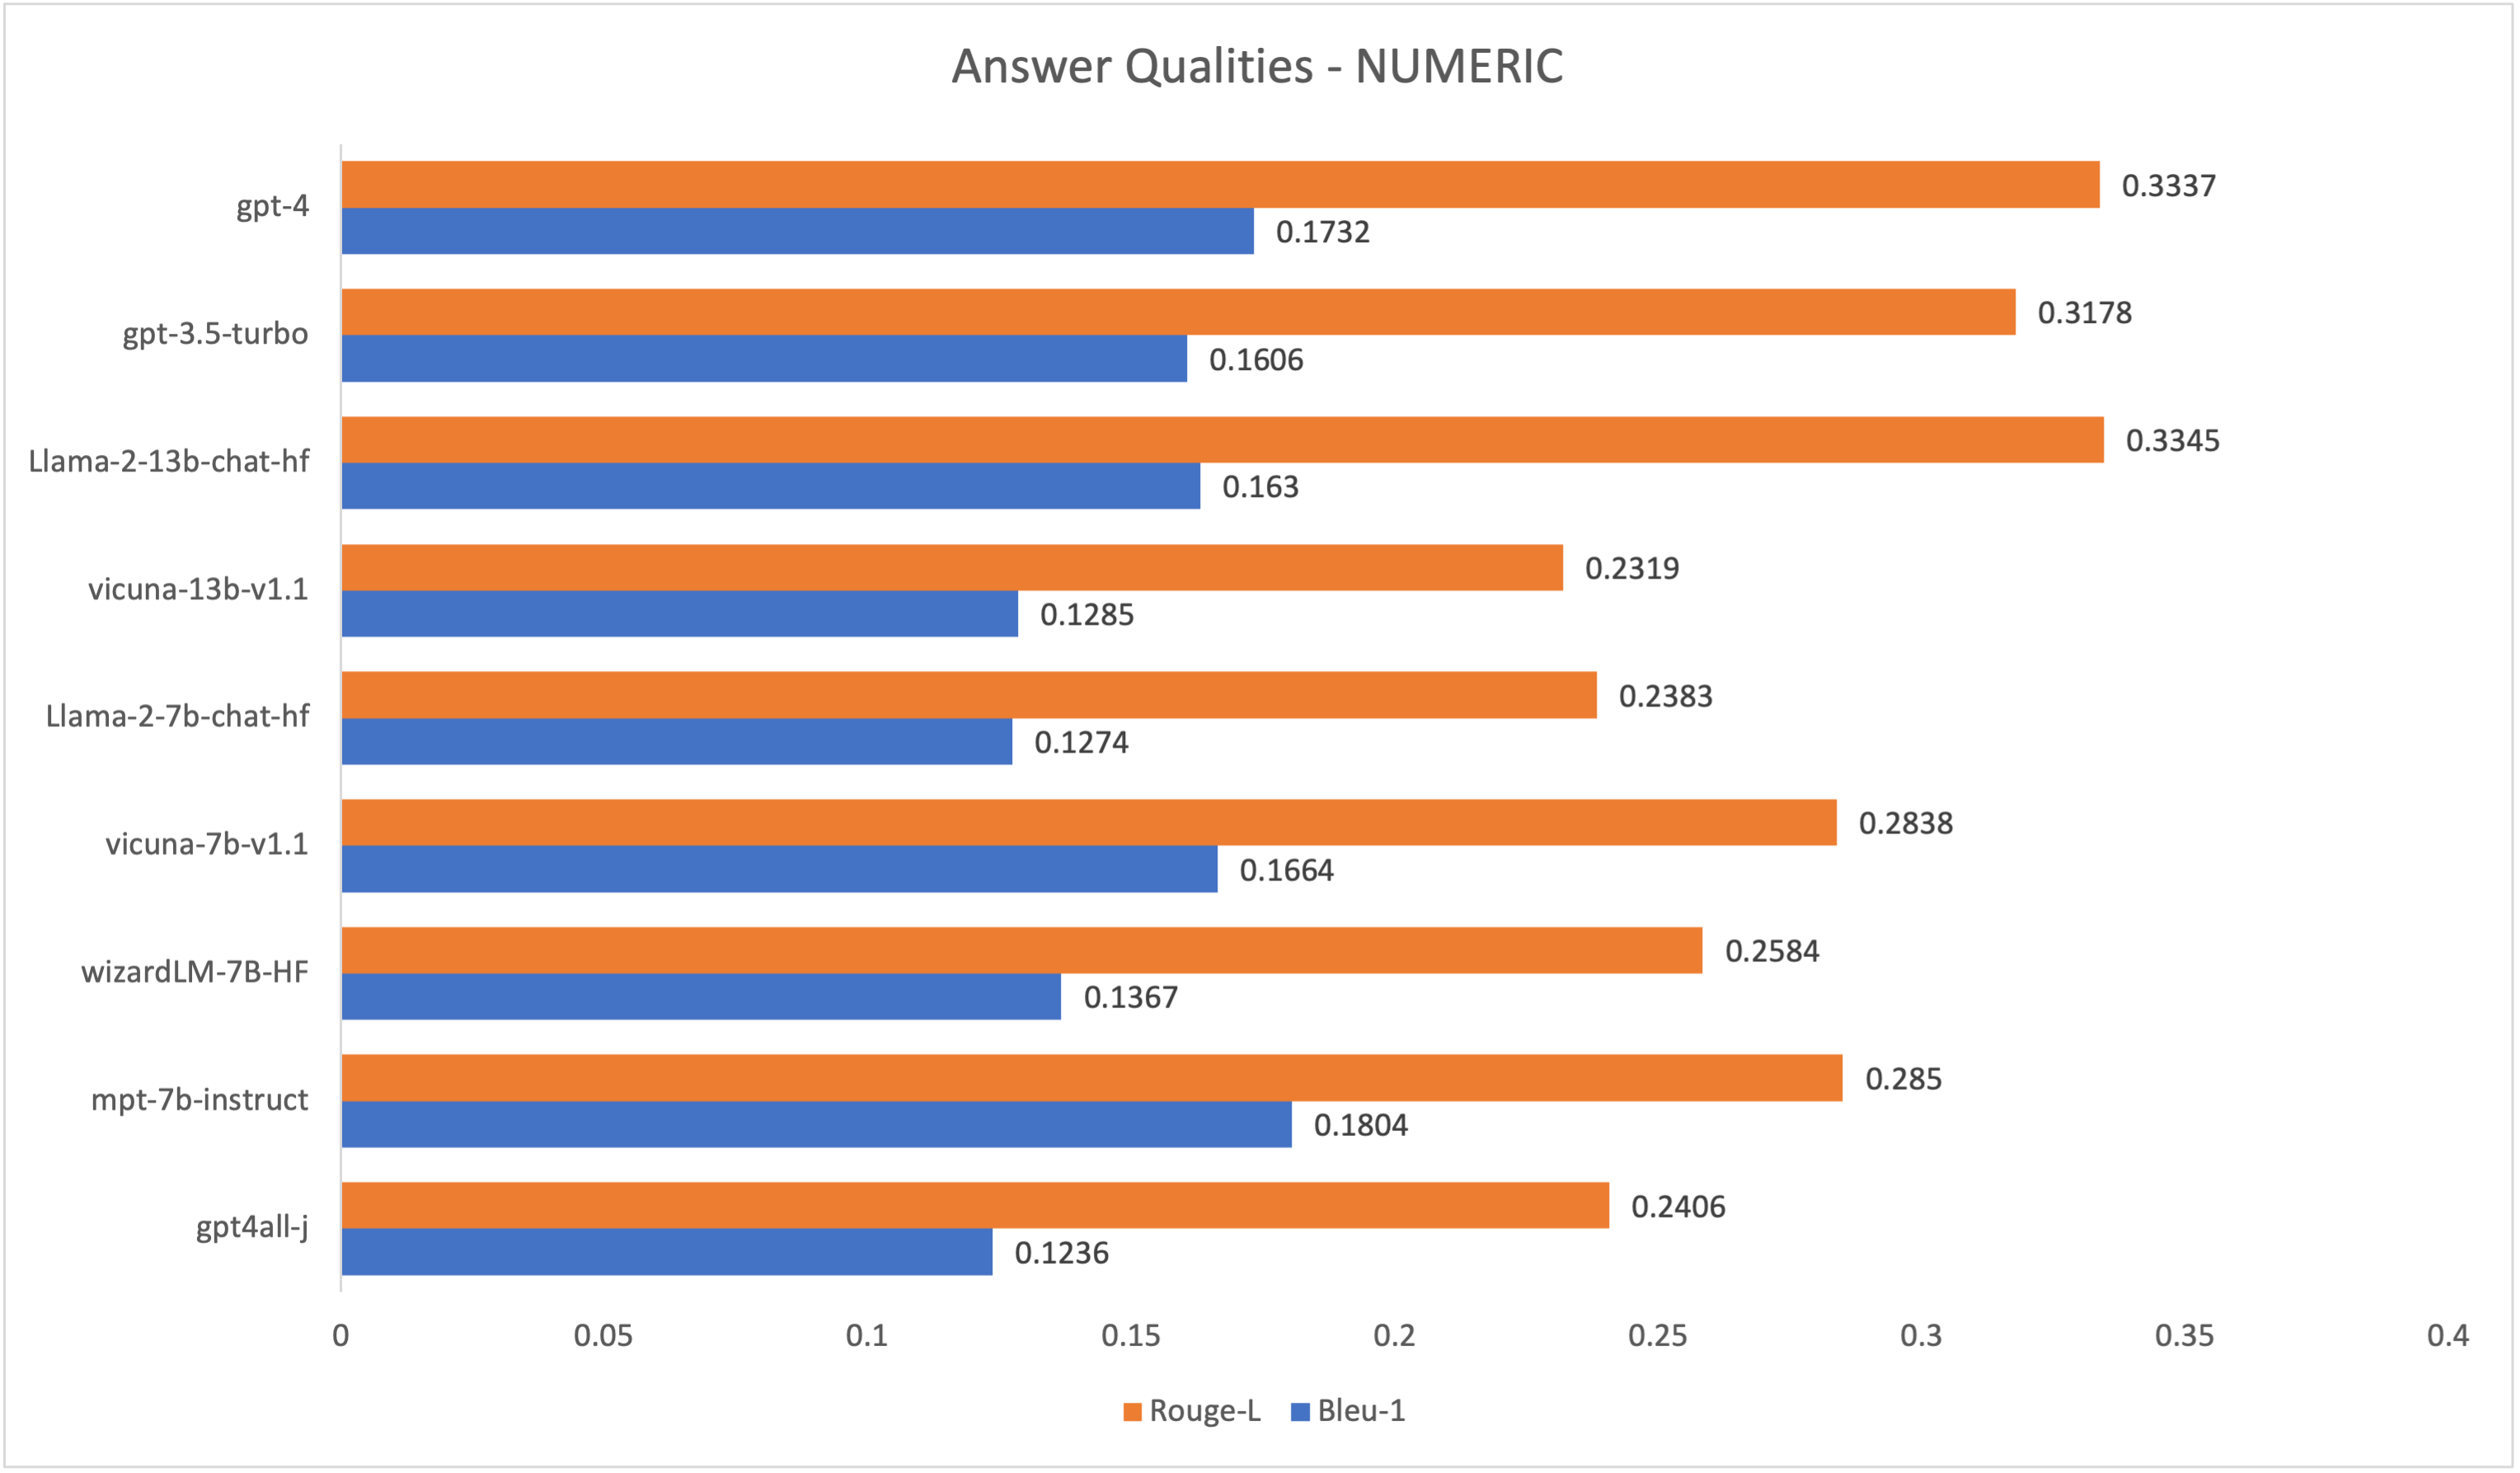
\includegraphics[width=0.48\textwidth]{figures/quality-numeric.png}} 
    \subfigure[PERSON]{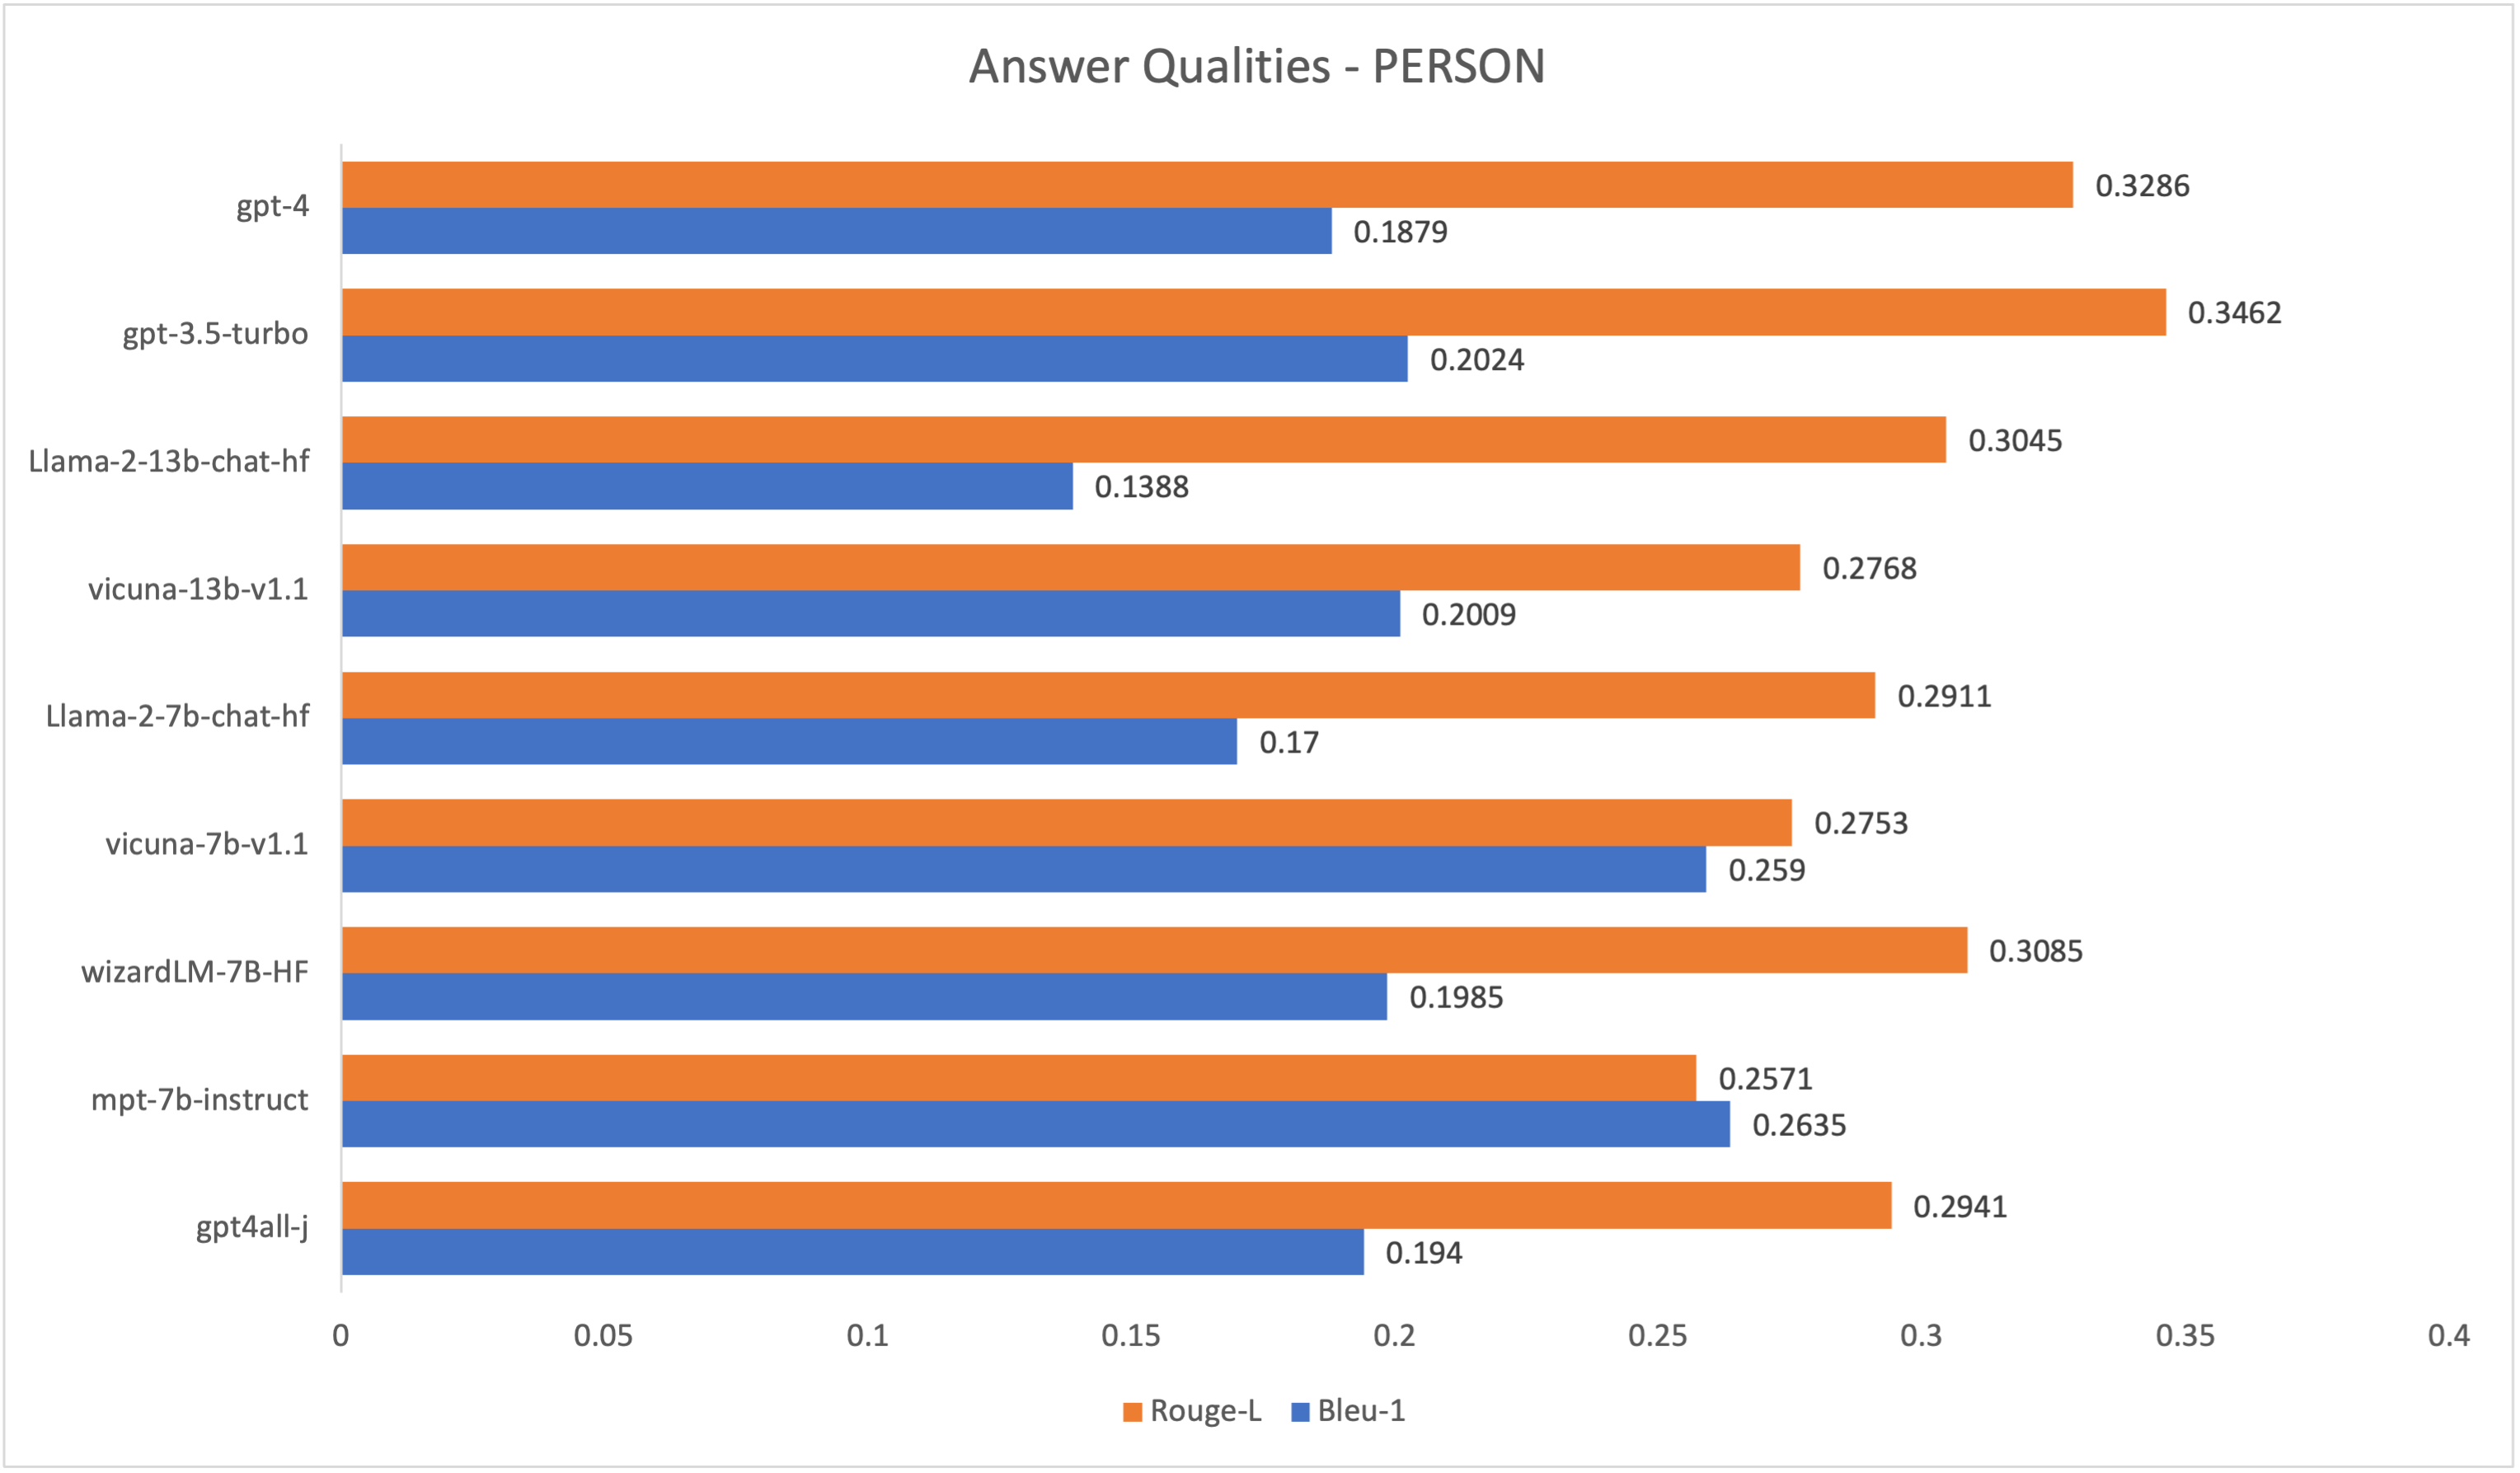
\includegraphics[width=0.48\textwidth]{figures/quality-person.png}} \\
    \subfigure[DESCRIPTION]{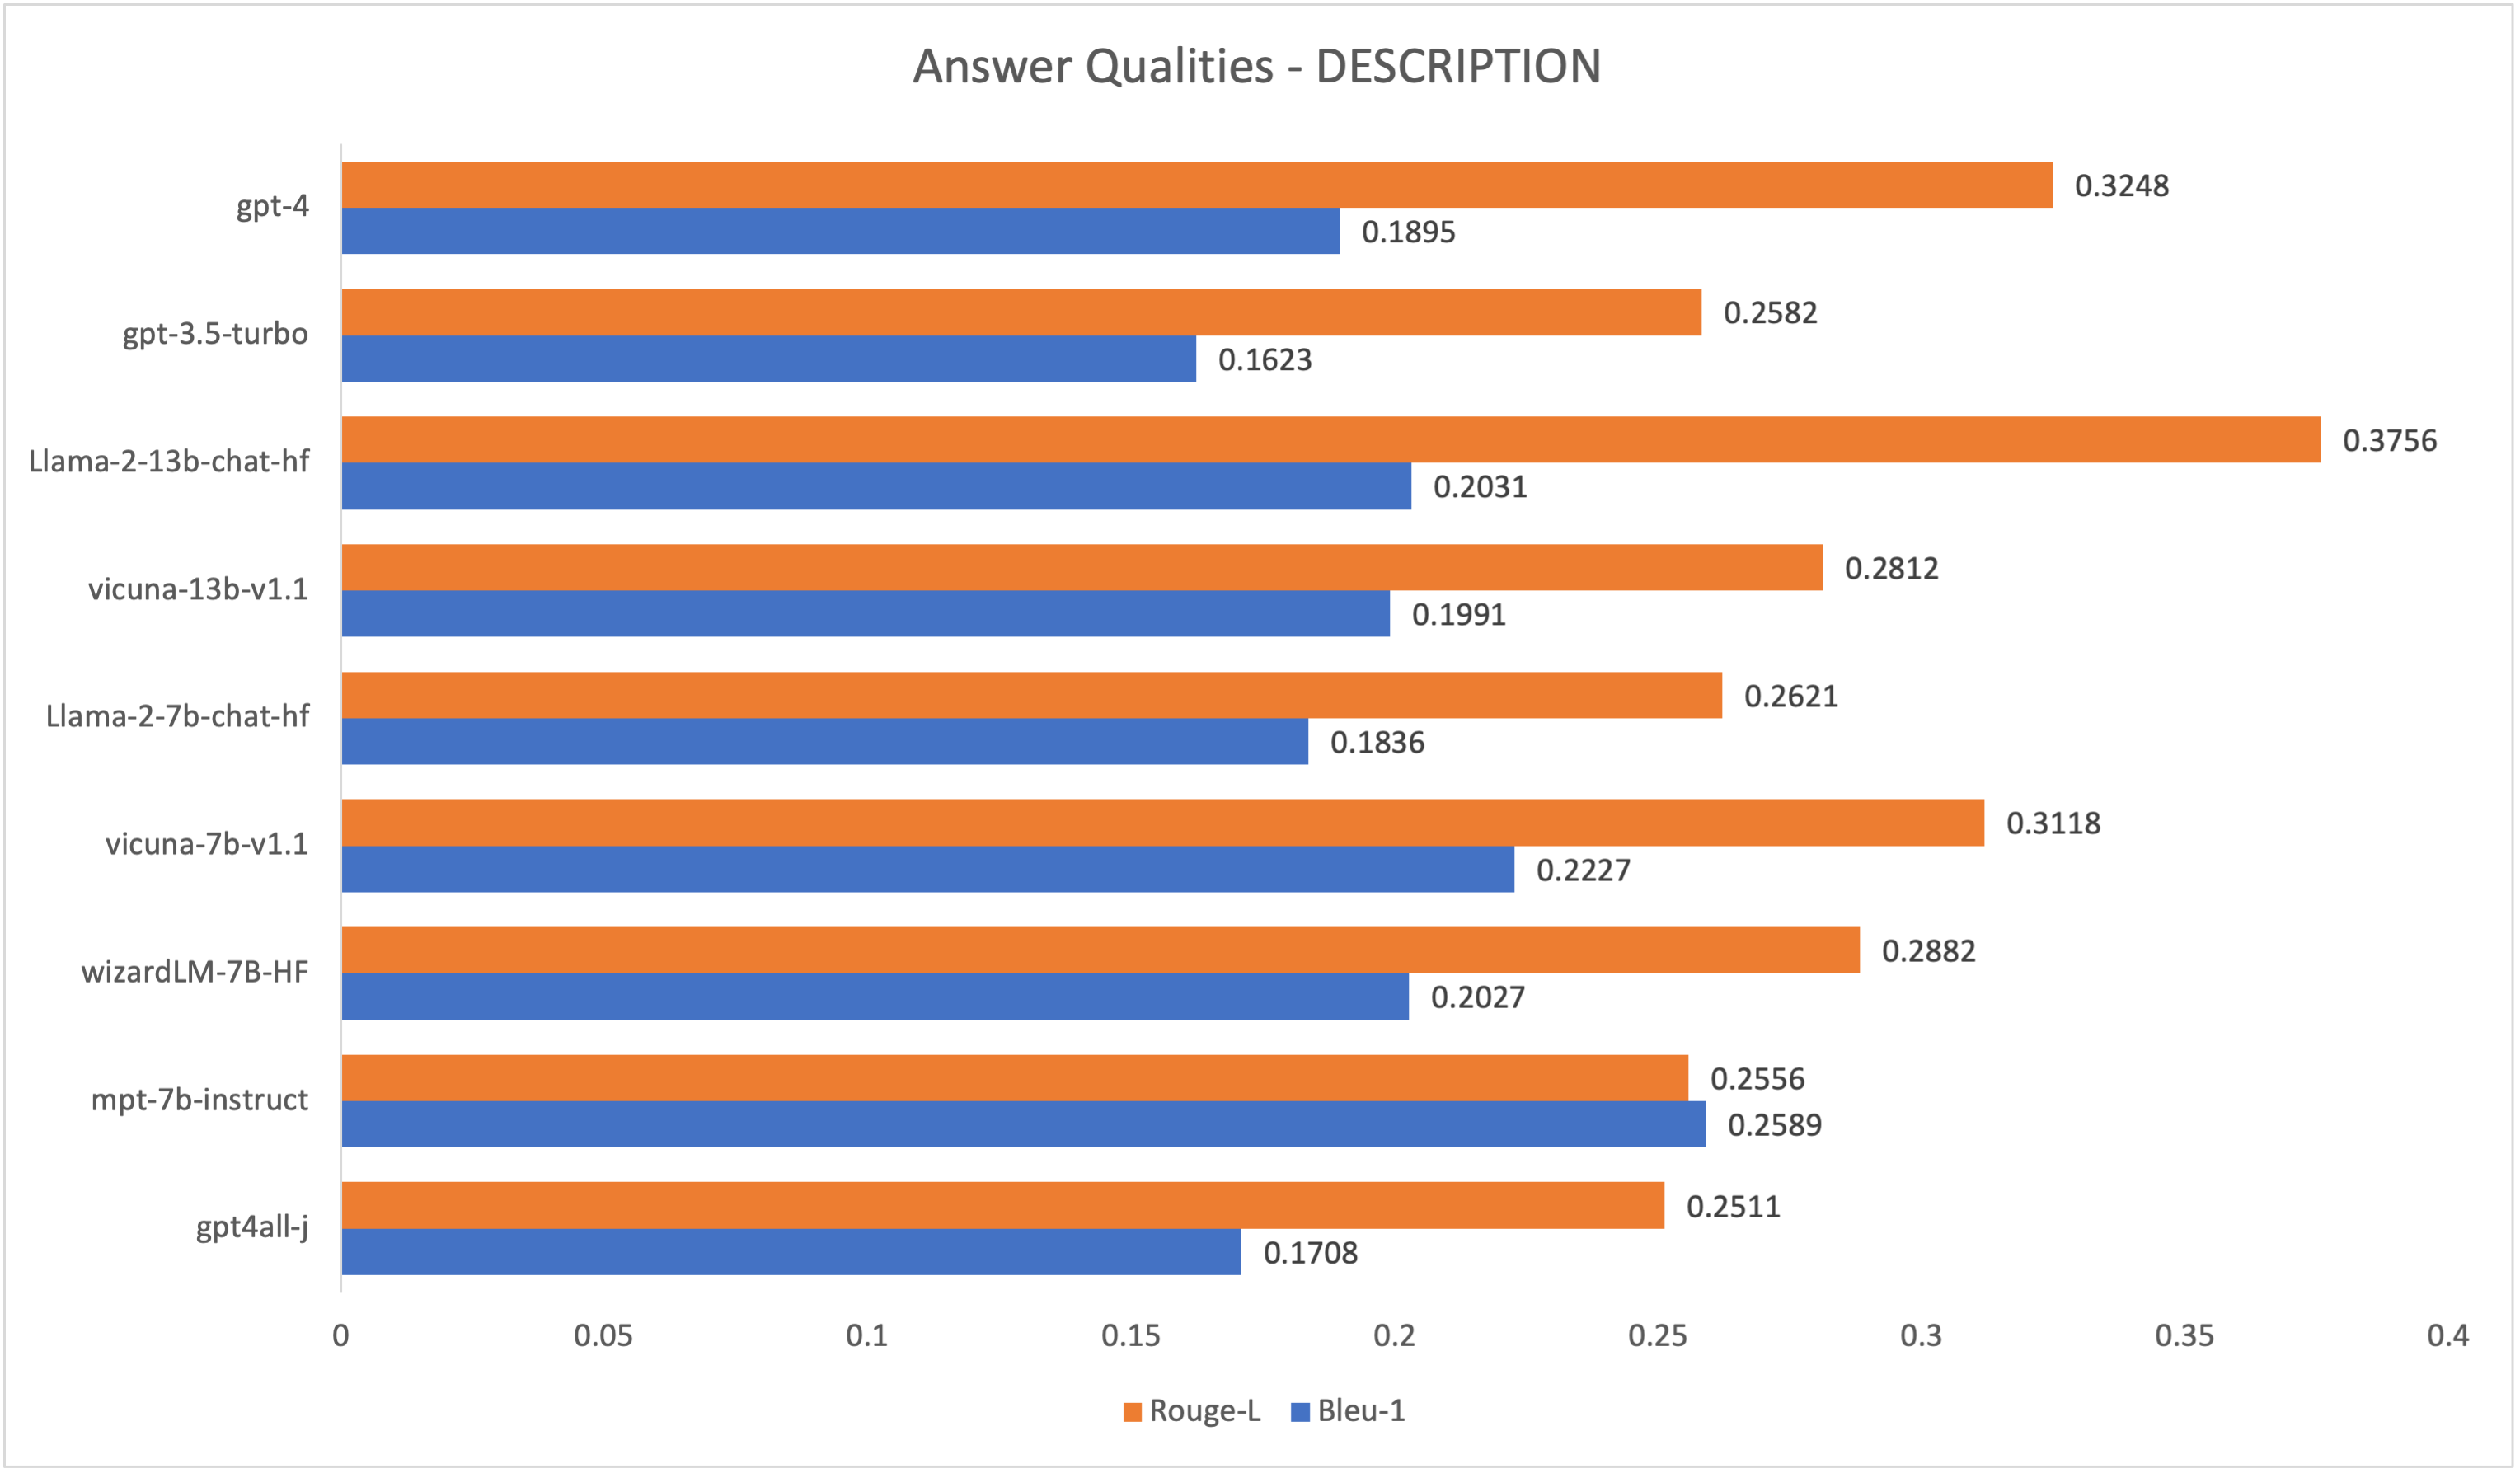
\includegraphics[width=0.48\textwidth]{figures/quality-description.png}} 
    \subfigure[ENTITY]{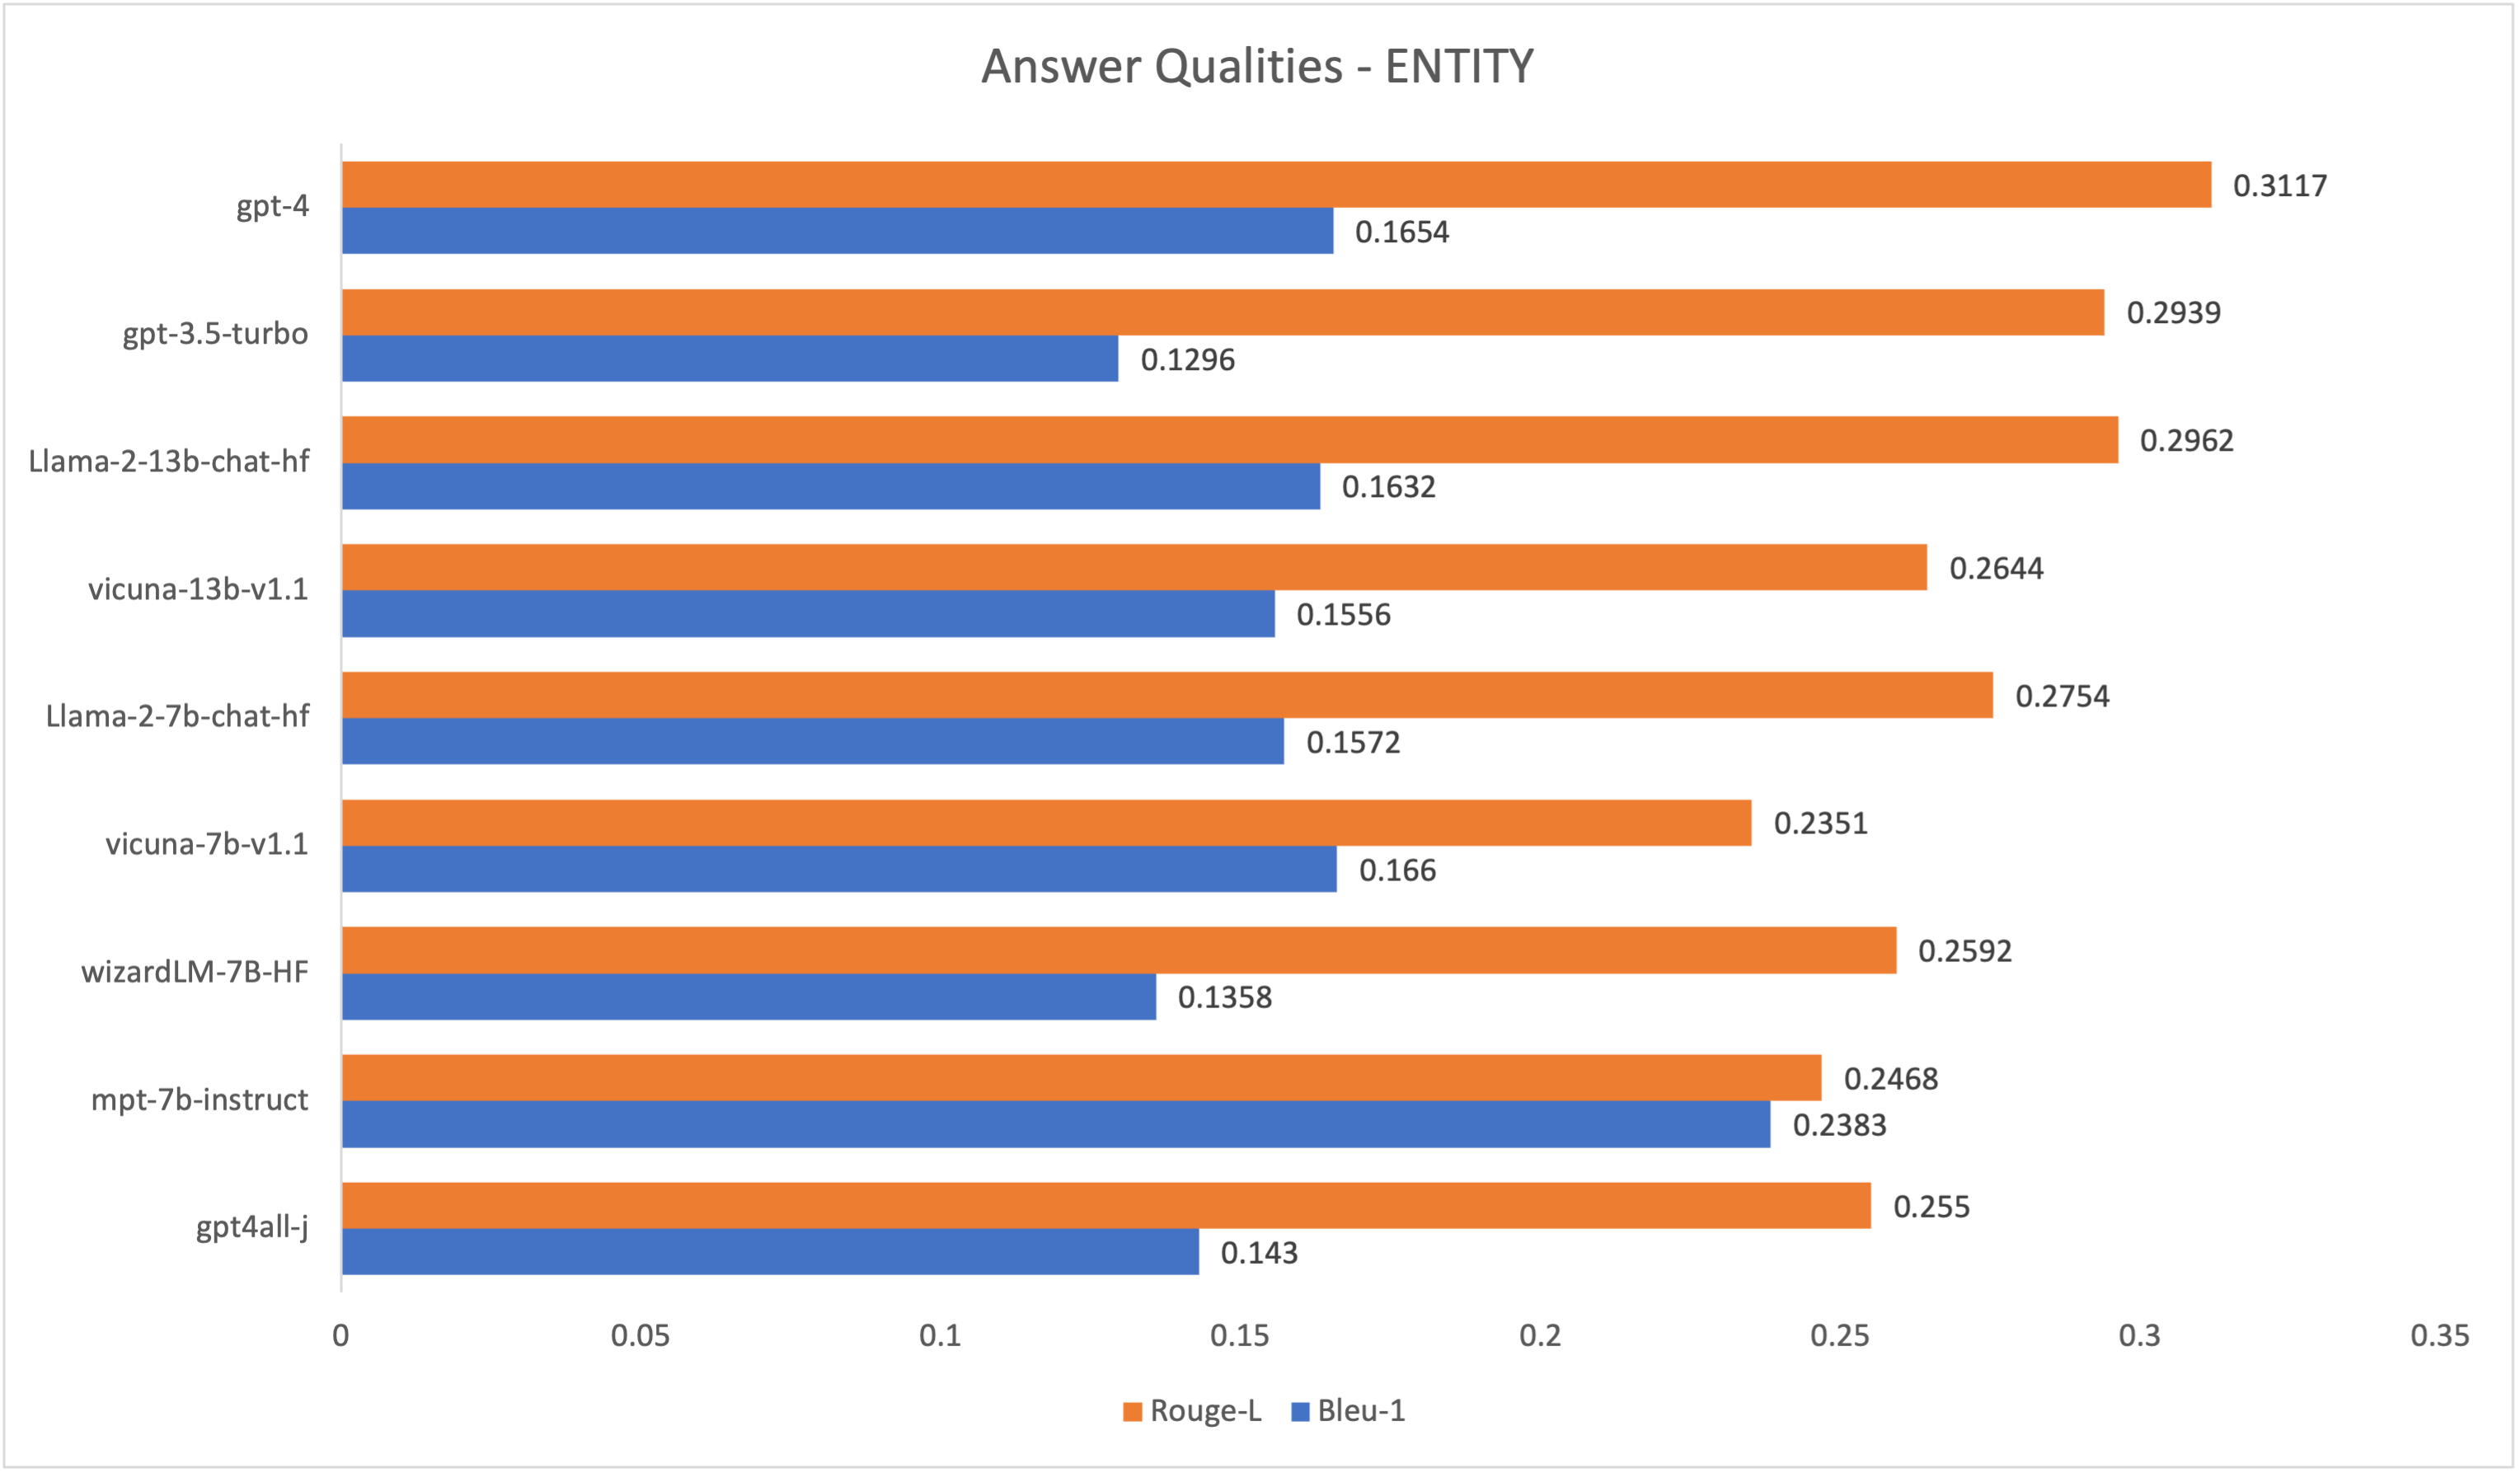
\includegraphics[width=0.48\textwidth]{figures/quality-entity.png}} 
\caption{Answer Qualities (running on Nvidia A40 GPUs)}
\label{fig:6}       % Give a unique label
\end{figure*}


\section{Research Discovery}
Within the scope of in-context learning, Llama-2 models perform on a level comparable to OpenAI's offerings. 
\begin{itemize}
    \item The Llama-2-13b-chat-hf model slightly edges out GPT-3.5-turbo in answer quality, but doesn't quite match up to GPT-4.
    \item When benchmarked on Nvidia A40 and L40 GPUs, Llama-2-13b-chat-hf shows faster inference speeds than GPT-4 but is slower than GPT-3.5-turbo. Using cutting-edge GPUs like Nvidia A100 or V100 might further optimize its performance. 
\end{itemize}

Comparatively, Llama-2 models stand out amongst other open-source LLMs.
\begin{itemize}
    \item With almost equivalent inference speeds, Llama-2-13b-chat-hf delivers superior answer quality compared to vicuna-13b-v1.1, despite the latter's claims of achieving over 90\% of the quality seen in OpenAI ChatGPT and Google Bard \footnote{\url{https://lmsys.org/blog/2023-03-30-vicuna/}}. 
    \item Llama-2-7b-chat-hf performs comparably to vicuna-7b-v1.1 and wizardLM-7b-HF in terms of speed and answer quality, and outperforms other 6B/7B LLMs.
\end{itemize}

In essence, our findings resonate with the claims made by Meta during the Llama-2 launch:
\begin{itemize}
    \item Llama-2-Chat models consistently outperform other open-source alternatives across diverse benchmarks. In terms of user evaluations focused on utility and safety, they match up well against industry-leading closed-source models like ChatGPT and PaLM. 
\end{itemize}

Currently, Llama-2 models represent the gold standard for commercially viable open-source LLMs. Yet, it's crucial to underscore Meta's licensing stipulation which mandates organizations with a monthly active user base exceeding 700 million to seek a dedicated license. Hence, it's imperative for large-scale enterprises to closely scrutinize these licensing stipulations before adopting Llama-2 models for business use.

\section{Conclusions}
This paper provides a comprehensive assessment of Llama 2's potential in the realm of in-context learning. Our findings highlight the comparable performance of Llama-2 models to leading OpenAI models, particularly in terms of answer quality. Moreover, we underscore Llama 2's potential to meet the requirements of commercial applications while emphasizing the importance of understanding and adhering to licensing terms, especially for enterprises with substantial user bases. Llama 2's emergence as a formidable open-source LLM signifies a promising future for NLP and AI-driven applications.

\bibliographystyle{IEEEtran}
\bibliography{ref}

\end{document}
